		\ifx \allfiles \undefined		%编译PPT时注释该行
\documentclass{book}
%%%%%%%%%%%%%%%%%%%%%%%%%%%%%%%%%%%%%%%%%
% 模板資訊:
% 模板名稱:Beamer
% 版本:1.0 (2023.07.09)
% 修改者:Ernie
% 編譯器:XeLaTeX
%
% 原始模板的資訊:
% 模板名稱:Beamer Presentation
% 作者:Vel (vel@latextemplates.com)
% 編譯器:XeLaTeX
% 授權:CC BY-NC-SA 4.0 (https://creativecommons.org/licenses/by-nc-sa/4.0/)
% 下載連結:https://www.LaTeXTemplates.com
%
% 製作本模板之目的:
% 為了讓 LaTeX 初學者能夠輕鬆地完成專業的學術簡報,因此我針對 Vel 製作的模板做了大幅度的修改及附上清楚明瞭的註解。
%
% 如果您有任何問題,可以透過 Email 聯繫我們:stateconlab@gmail.com
% 
% p.s. 也別忘了關注我們的 YouTube、IG 和 Medium 喔!
% 1. YouTube:https://www.youtube.com/@StatEconLab
% 2. IG:https://www.instagram.com/stateconlab
% 3. Mediun:https://medium.com/@stateconlab
%%%%%%%%%%%%%%%%%%%%%%%%%%%%%%%%%%%%%%%%%

%----------------------------------------------------------------------------------------
%	封包與文檔配置
%----------------------------------------------------------------------------------------

\usepackage[space,noindent]{ctex}

% 自訂字體顏色的封包
\usepackage{xcolor} 

%% 自訂顏色

\definecolor{pbblue}{HTML}{0A75A8}% color for the progress bar and the circle
% 數學工具及符號
%\usepackage{mathtools, amsmath, amsfonts, amsthm, latexsym} 

% 分別將數學符號間的間隔加大及加粗
%\usepackage{newtxtext,newtxmath}

% 圖表自動編號的封包
%\usepackage{caption} 

%% 設定自動編號
%\setbeamertemplate{caption}[numbered]

%% 設定圖表編號及標籤的字體大小及字形
%\captionsetup[figure]{font=small, labelfont=md}
%\captionsetup[table]{font=small, labelfont=md}

% 導入圖形與表格的封包
%\usepackage{graphicx}  % \scalebox{} 可用於將過大的表格縮小
%\usepackage{booktabs}

% 排列多個子圖形的封包
%\usepackage{subfigure} 

% 允許表格的一格能多列呈現的封包
%\usepackage{multirow} 

% 可指定表格排版的封包
%\usepackage{array}

% 翻轉表格的封包
%\usepackage{lscape} 

% 序列標號
%\usepackage{enumerate} 

% 繪圖封包 (用於添加浮水印)
\usepackage{tikz}

% 引注參考資料
%\usepackage{natbib}

% 註釋掉大部分的封包
%\usepackage{comment}

\usetikzlibrary{shapes,fit,calc,positioning}

% 設定中文的標籤
%\renewcommand{\figurename}{圖} 
\renewcommand{\tablename}{表} 

%----------------------------------------------------------------------------------------
%	排版形式 (擇一,不選等同選擇默認的排版形式)
%----------------------------------------------------------------------------------------

%\mode<presentation>{
%\usetheme{default}
%\usetheme{AnnArbor}
%\usetheme{Antibes}
%\usetheme{Bergen}
%\usetheme{Berkeley}%演示主题为侧边导航条
%\usetheme{Berlin}
\usetheme{Boadilla}%蓝色主题
%\usetheme{CambridgeUS}
%\usetheme{Copenhagen}
%\usetheme{Darmstadt}
%\usetheme{Dresden}
%\usetheme{Frankfurt}
%\usetheme{Goettingen}
%\usetheme{Hannover}
%\usetheme{Ilmenau}
%\usetheme{JuanLesPins}
%\usetheme{Luebeck}
%\usetheme{Madrid}
%\usetheme{Malmoe}
%\usetheme{Marburg}
%\usetheme{Montpellier}
%\usetheme{PaloAlto}
%\usetheme{Pittsburgh}
%\usetheme{Rochester}
%\usetheme{Singapore}
%\usetheme{Szeged}
%\usetheme{Warsaw}

%----------------------------------------------------------------------------------------
%	外框形式 (擇一,不選等同選擇默認的外框形式)
%----------------------------------------------------------------------------------------

%\useoutertheme{default}
%\useoutertheme{infolines}
%\useoutertheme{miniframes}
%\useoutertheme{smoothbars}
%\useoutertheme{sidebar}
%\useoutertheme{split}
%\useoutertheme{shadow}
%\useoutertheme{tree}
%\useoutertheme{smoothtree}

%----------------------------------------------------------------------------------------
%	外框的自訂義調整 
%----------------------------------------------------------------------------------------

% 外框上緣的字 (fg) 為黑色,背景 (bg) 為白色。
%\setbeamercolor{section in head/foot}{fg=white, bg=black} 

% 外框上緣顯示的章節(section)頁數標籤是否關閉
%\setbeamertemplate{mini frames}{}   

% 調整外框形式的字體大小
%\setbeamerfont{headline}{size=\scriptsize}
%\setbeamerfont{footline}{size=\scriptsize}

% 取消右下方的跳轉工具列
\setbeamertemplate{navigation symbols}{} 

%% 自定義1:外框下緣僅出現名字及頁碼
%\setbeamertemplate{footline}
%{\leavevmode%
%\hbox{%
%\begin{beamercolorbox}[wd=0.5\paperwidth,ht=3ex,dp=1ex,leftskip=2ex]%
%{author in head/foot}%
%{\footnotesize\textbf{\insertshortauthor}}%
%\end{beamercolorbox}%
%\begin{beamercolorbox}[wd=0.5\paperwidth,ht=3ex,dp=1ex,right]%
%{author in head/foot}%
%\footnotesize \textbf{{\insertframenumber{} / \inserttotalframenumber\hspace*{2ex}}} %頁碼控制選項
%\end{beamercolorbox}%
%}}

%% 自定義2:清除外框下緣但僅出頁碼
%\setbeamertemplate{footline}[page number] 

%% 自定義3:清除外框下緣
%\setbeamertemplate{footline}[] 

%----------------------------------------------------------------------------------------
%	顏色主題 (擇一,不選等同選擇默認的顏色主題)
%----------------------------------------------------------------------------------------

%\usecolortheme{default}
%\usecolortheme{albatross}
%\usecolortheme{beaver}
%\usecolortheme{beetle}
%\usecolortheme{crane}
%\usecolortheme{dolphin}
%\usecolortheme{dove}
%\usecolortheme{fly}
%\usecolortheme{lily}
%\usecolortheme{orchid}
%\usecolortheme{rose}
%\usecolortheme{seagull}
%\usecolortheme{seahorse}
\usecolortheme{whale}%颜色主题为
%\usecolortheme{wolverine}

%----------------------------------------------------------------------------------------
%	顏色主題的自訂義調整 
%----------------------------------------------------------------------------------------

% 全文的主題色 (可以特別針對報告對象或機構的代表色調整!)
%\setbeamercolor{structure}{fg=Myblue} 

% 封面頁中標題區塊的底色及字體顏色
%\setbeamercolor{title}{bg=green, fg=black} 

% 各頁標題區塊的底色及字體顏色
%\setbeamercolor{frametitle}{bg=white,fg=black} 

% 全文的內文顏色
%\setbeamercolor{normal text}{fg=orange}

% 數學區塊的標題顏色 
%\setbeamercolor{block title}{bg=blue,fg=yellow} 

% 數學區塊的內文顏色 
%\setbeamercolor{block body}{bg=green,fg=red} 

% 警示文字的顏色
%\setbeamercolor{alerted text}{fg=red} 

%----------------------------------------------------------------------------------------
%	enumerate 及 item 的形狀
%----------------------------------------------------------------------------------------

%\useinnertheme{rounded} % 圓球 (3D)
%\useinnertheme{circles} % 圓形 (2D)
%\useinnertheme{rectangles} % 方形
%\useinnertheme{triangle} % 三角形
%\useinnertheme{inmargin} % 插入邊沿
%\setbeamertemplate{itemize items}[triangle]

%----------------------------------------------------------------------------------------
%	自訂 item 的顏色
%----------------------------------------------------------------------------------------

%\setbeamercolor{item projected}{bg=red}

%----------------------------------------------------------------------------------------
%	個人化的設置及細節調整
%----------------------------------------------------------------------------------------

% 設定頁面邊界
%\setbeamersize{text margin left=0.6cm, text margin right=0.6cm}
%\special{papersize=\the\paperwidth,\the\paperheight}
%\providecommand{\tabularnewline}{\\}
%}

%----------------------------------------------------------------------------------------
%	個人化的背景調控
%----------------------------------------------------------------------------------------

% 背景照片設置
%\setbeamertemplate{background}{\includegraphics[height=\paperheight]{Fig/Background.png}}

% 浮水印設定
%\usebackgroundtemplate{%
%	\tikz[overlay, remember picture] % 讓 logo 能每頁都顯示
%	\node[opacity=0.3, below=-1.25cm, at=(current page.center)] % 調整透明度 (opacity) 及浮水印的位置
%	{\includegraphics[scale = 0.14]{Fig/nthulogo.png}}; % 載入 logo 及調整大小
%	}

\begin{document}
		\else						%编译PPT时注释该行
		%\newpage
		\fi						%编译PPT时注释该行
\watermark{50}{9}{热工班组}
\chapter[2024年03月份技术培训考试]{	\hspace*{-0.3em}\biaoti{2024}{03}{热工专业}}
姓名:\uline{ \ \  \  \ \ \ \ \ \ \ \ \ \ \ \ \ \ }\hfill 得分:\uline{ \ \  \  \ \ \ \ \ \  \ \ \ \ \ \ }
%\zysx
\section{\xzt{5}{2}{10}}
\begin{enumerate}
\item 我厂3汽号轮机的AST电磁阀供电电压是\xz{D}。
\xx{220ACV}{220DCV}{380AVC}{24DCV}
\item 我厂3汽号轮机的AST电磁阀供电端子保险是\xz{C}。
\xx{0.2A}{1A}{3A}{0.1A}
\item 我厂4汽号轮机的AST电磁阀供电电压是\xz{B}。
\xx{220ACV}{220DCV}{380AVC}{24DCV}
\item 我厂4汽号轮机的主汽门电磁阀(磁力断路油门)供电电压是\xz{A}。
\xx{220ACV}{220DCV}{380AVC}{24DCV}
\item 我厂次高压汽轮机ETS系统S7 200PLC与DEH系统之间数据传递采用哪种方式\xz{D}。
\xx{OPC通讯}{RS 232/485通讯}{4-20mA}{PROFIBUS通讯}
\end{enumerate}
\section{\tkt{4}{2}{34}}
\begin{enumerate}
	\setcounter{enumi}{5}
	\item 我厂次高压汽轮机ETS系统控制器使用的PLC型号为CPU 226 CN AC/DC/RLY,其中AC/DC/RLY分别对应着\tk{电源电压}/\tk{输入电压}/\tk{输出电压},AC表示交流\tk{220V},DC表示\tk{直流24V},RLY表示\tk{继电器输出},ETS控制系统通过\tk{并联输入、输出}实现控制系统冗余。
\item 汽轮机常规的超速保护有\tk{OPC}、\tk{电超速}、\tk{机械超速}三种。
\item 我厂次高压汽轮机正常运行时,汽轮机的润滑油压由\tk{主油泵}供给,当润滑油压降低时应自动联锁启动\tk{交流润滑油泵}。
\item 电涡流传感器系统的三个组成部分是\tk{探头}、\tk{延长电缆}、\tk{前置器}。
\item 我厂4号汽轮机高调门伺服阀为\tk{单级}、\tk{直驱}电液伺服阀。
\end{enumerate}
\section{\stt{16}}
\begin{enumerate}
	\setcounter{enumi}{10}
	\item 下图为西门子S7200 PLC控制器,在图中标出控制器上各部件名称?\\
		\tupian{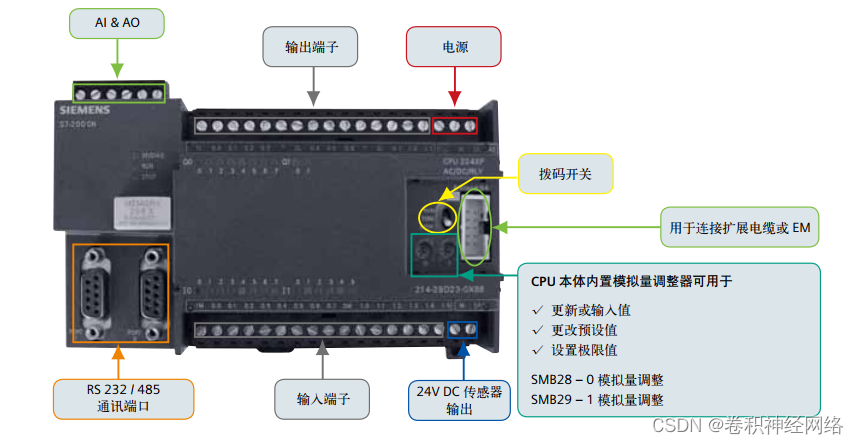
\includegraphics[angle=0,width=500pt,trim=0 0 0 0,clip]{picture/200plc_da.png}}{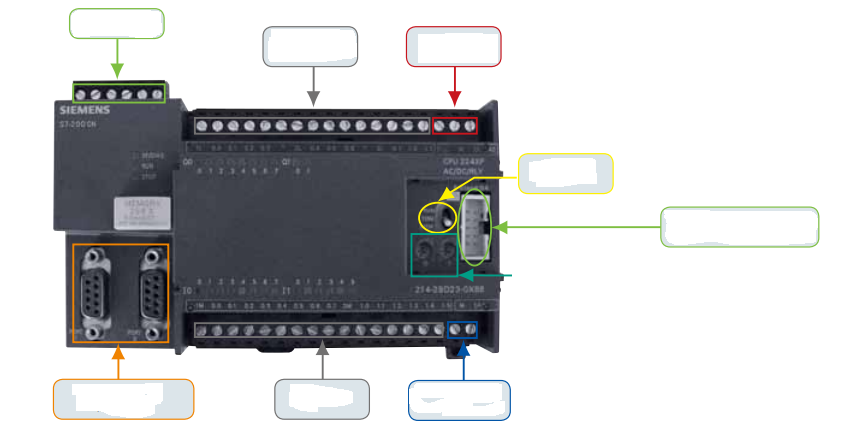
\includegraphics[angle=0,width=500pt,trim=0 0 0 0,clip]{picture/200plc.png}}

%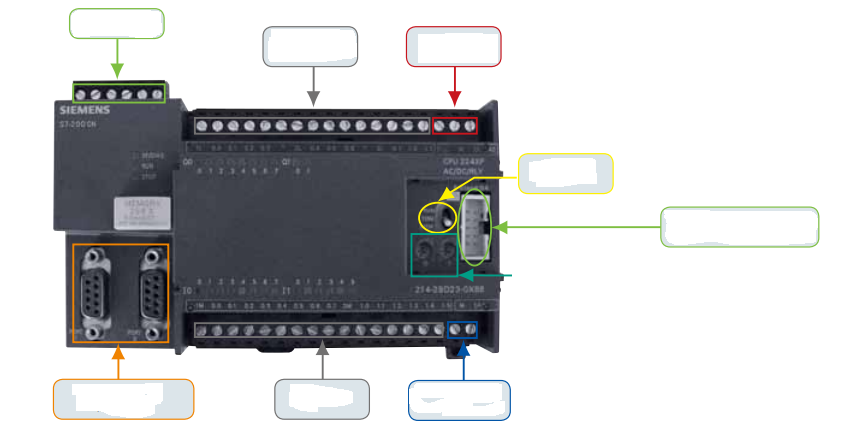
\includegraphics[angle=0,width=500pt,trim=0 0 0 0,clip]{picture/200plc.png}%答案需要替换下图片


\end{enumerate}
\section{\jdt{40}}
\begin{enumerate}
	\setcounter{enumi}{11}
\item 我厂次高压汽轮机ETS保护有哪些?其中DCS请求停机保护包含哪些?DEH请求停机保护包含哪些?\fenzhi{20}
\wdt[6]{答:\\
汽轮机轴承振动大:现场8支电涡流探头通过前置器输出电压信号至TSI系统,TSI系统对应卡件分别输出4-20mA信号至DCS系统后进行逻辑判断后触发DCS停机信号
主油箱油位低:现场油位测量装置通过TSI机柜内变送器输出信号至TSI系统,TSI系统对应卡件分别输出4-20mA信号至DCS系统后进行逻辑判断后触发DCS停机信号
轴承金属温度高与回油温度高:现场热电阻元件输出信号至TSI系统对应卡件后输出4-20mA信号至DCS系统后进行逻辑判断后触发DCS停机信号
}
\item 我厂净烟气二氧化硫分析仪模拟量输出为双量程自动切换输出,配合模拟量量程切换有一个高低量程开关量输出,即仪表显示小于50时模拟量通道量程为0-50,高低量程开关量输出为0,大于50时模拟量通道量程自动切为0-200,高低量程开关量输出变为1,而DCS系统AI通道没有切换功能,在DCS系统如何正常显示分析仪二氧化硫数据\fenzhi{20}
\wdt[6]{答:\\
汽轮机轴承振动大:现场8支电涡流探头通过前置器输出电压信号至TSI系统,TSI系统对应卡件分别输出4-20mA信号至DCS系统后进行逻辑判断后触发DCS停机信号
主油箱油位低:现场油位测量装置通过TSI机柜内变送器输出信号至TSI系统,TSI系统对应卡件分别输出4-20mA信号至DCS系统后进行逻辑判断后触发DCS停机信号
轴承金属温度高与回油温度高:现场热电阻元件输出信号至TSI系统对应卡件后输出4-20mA信号至DCS系统后进行逻辑判断后触发DCS停机信号
}
\end{enumerate}
		\ifx \allfiles \undefined
\end{document}
\fi
